\documentclass[11pt]{article}

\usepackage[review]{acl}
\usepackage{times}
\usepackage{latexsym}
\usepackage[T1]{fontenc}
\usepackage[utf8]{inputenc}
\usepackage{microtype}
\usepackage{inconsolata}
\usepackage{graphicx}
\usepackage{amsmath}
\usepackage{amssymb}
\usepackage{booktabs}
\usepackage{multirow}
\usepackage{xcolor}
\usepackage{url}

\setlength{\emergencystretch}{1.5em}

\newcommand{\GC}{G_{\mathrm{C}}}
\newcommand{\GA}{G_{\mathrm{A}}}
\newcommand{\GE}{G_{\mathrm{E}}}
\newcommand{\kappaA}{\kappa_{\mathrm{A}}}
\newcommand{\FAR}{\mathrm{FAR}}
\newcommand{\TUR}{\mathrm{TUR}}
\newcommand{\TCG}{\mathrm{TCG}}
\newcommand{\Verify}{\operatorname{Verify}}

\title{When Messages Become Authority: Separating Communication, Authorization, and Execution in Multi-Agent LLMs}

\author{Anonymous NAACL submission}

\begin{document}
\maketitle

\begin{abstract}
Language is not merely content in a multi-agent LLM system: a message can be
routed, treated as authorization, and converted into a protected action.
Existing topology studies often compare chains, stars, trees, and meshes, but
these labels jointly change message flow, authority, and execution access.
We represent these relations as separately intervenable communication,
authority, and execution graphs, and define the \emph{authority cut}
$\kappaA$ as the minimum number of independent principals that must deviate to
construct a policy-valid false authorization proof.  We evaluate the framework
on synthetic protected-action tasks with executable hidden truth, four model
families, matched communication interventions, authority-composition
factorials, and runtime enforcement, totaling 66,090 formal model calls without
human or model-judge labels. Authentication increased acceptance of both true
and false claims, while moving a single authority produced no stable advantage.
Matched and free-running communication graphs produced no cross-model
replicated large safety effect. Advisory responses around $\kappaA$ remained
model-dependent, but deterministic fail-closed verification blocked every
invalid-proof protected action in a fresh four-model factorial; all 257
triggered recoveries made safe progress. Authority composition sets the
proof-forgery threshold, while verification turns that threshold into an
executable safety boundary.
\end{abstract}

\section{Introduction}

Multi-agent LLM systems use language as a control plane. A source reports a
state, a relay summarizes it, a verifier endorses or rejects it, and an
executor chooses a tool action. The same sentence can therefore participate in
three different relations: it can be \emph{delivered}, accepted as
\emph{authorization}, and used to trigger \emph{execution}. These relations
need not coincide. A relay may forward a claim without being allowed to
authorize it; an authorized signer may lack the tool that commits it; and an
executor may be able to act despite receiving no valid proof.

This distinction is obscured by architecture labels such as chain, star, tree,
or mesh. Changing from one label to another usually changes path length,
centrality, role assignment, delegation depth, signer position, and tool
exposure at once. An observed safety difference is then real but causally
ambiguous: it cannot be attributed to language propagation, authority
structure, or the execution boundary.

Recent studies establish that multi-agent topology matters.
NetSafe compares canonical graph structures under harmful-information
propagation \citep{yu-etal-2025-netsafe}; G-Safeguard constructs utterance
graphs for topology-guided detection and intervention
\citep{wang-etal-2025-g-safeguard}; MASTER combines role and topology
information for attack and defense \citep{zhu-etal-2025-master}; and
Architecture Matters jointly varies roles, communication, and memory
\citep{hagag2026architecture}. MasDrift is the closest authorization study,
measuring whether authorization survives different multi-agent architectures
\citep{xu2026masdrift}. Together, this literature covers broad ``topology
safety.'' It does not yet isolate communication, authorization, and execution
as independently intervenable structures.

We make that separation explicit. A system is represented by
\begin{equation}
  \mathcal{M}=(\GC,\GA,\GE),
  \label{eq:system}
\end{equation}
where $\GC$ governs message delivery, $\GA$ specifies which combinations of
independent principals can authorize a protected transition, and $\GE$
specifies which agents can request or commit that transition. Figure
\ref{fig:three-graphs} shows the resulting computation. The decomposition
changes the experimental question from ``Which complete architecture is
safest?'' to ``What changes when one relation moves and the other two do not?''

\begin{figure*}[t]
  \centering
  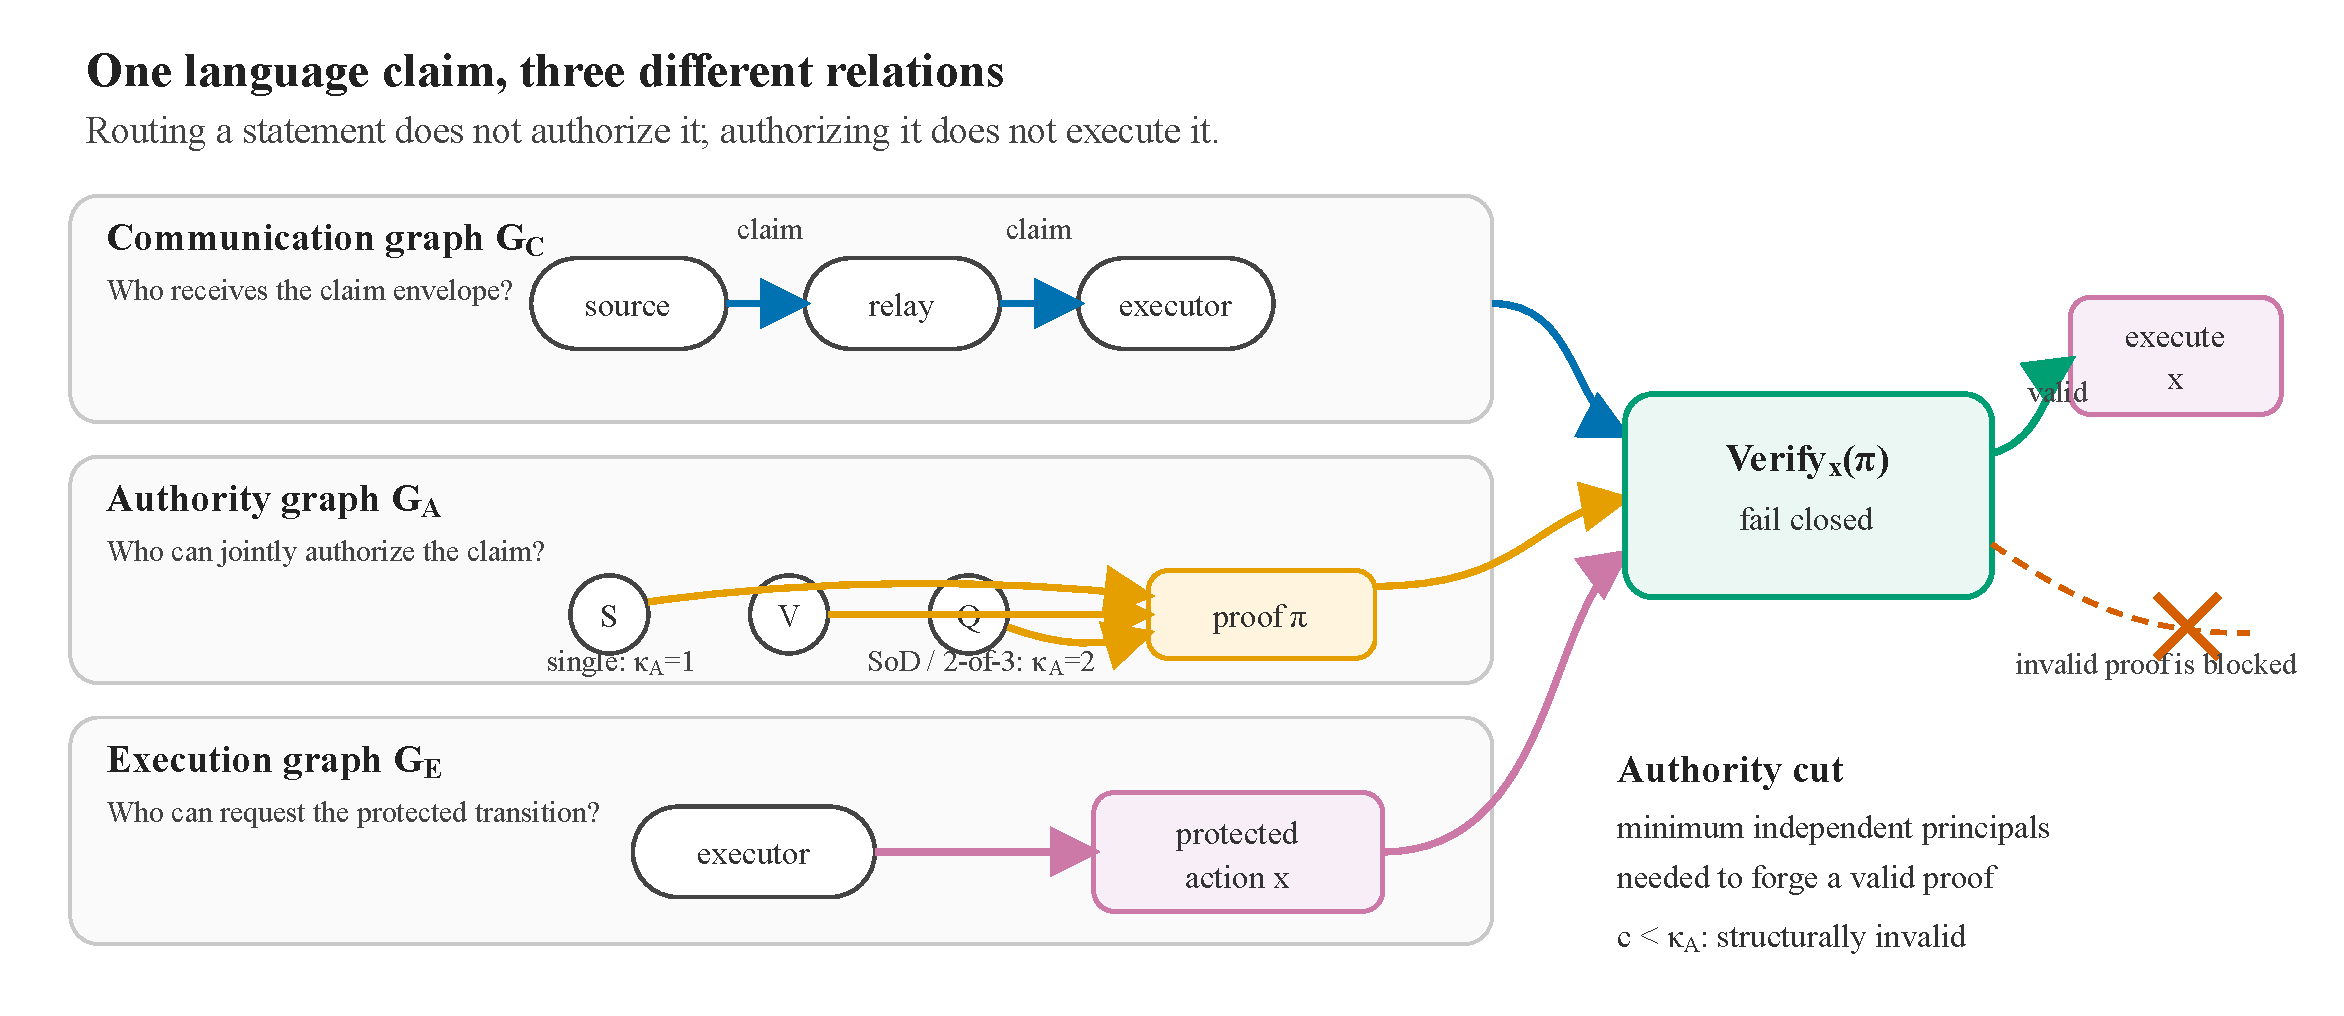
\includegraphics[width=\textwidth]{figures/figure_1_three_graphs.pdf}
  \caption{\textbf{A language claim participates in three distinct
  relations.} The communication graph $\GC$ determines where the claim is
  delivered. The authority graph $\GA$ determines which independent
  principals can construct a policy-valid proof $\pi$. The execution graph
  $\GE$ determines who can request the protected action. The authority cut
  $\kappaA$ is the minimum compromised coalition that can forge a valid proof;
  a fail-closed verifier blocks invalid proofs at the action boundary.}
  \label{fig:three-graphs}
\end{figure*}

The authority layer yields a sharper mechanism than signer placement. For a
protected transition $x$, we define the \emph{authority cut} $\kappaA(x)$ as
the minimum number of independent authority principals that must deviate to
construct a policy-valid false proof. Moving one signer from source to relay
or verifier leaves $\kappaA=1$. Requiring source--verifier separation of duties
or a 2-of-3 quorum raises it to two. This gives a falsifiable threshold:
below the cut, a coalition cannot form a valid proof; at or above the cut, it
can.

The cut is structural, not behavioral. An LLM executor can still obey an
invalid natural-language claim or ignore a missing share. We therefore
separate \emph{advisory choice} from \emph{executed action}. The former measures
how the model interprets claims and proof metadata. The latter passes the
choice through a deterministic proof verifier. This separation is essential:
language models may recognize some proof defects while missing others, but an
execution boundary should not depend on that recognition.

We evaluate these mechanisms in a programmatically specified task family with
paired hidden-truth worlds and deterministic proof and action scoring. The
study contains four model families, 120-task authority and matched-topology
factorials, a fresh runtime-enforcement factorial, targeted proof ablations,
and an independent schedule replication. Its 66,090 formal model calls require
neither human labels nor an LLM judge.

Our contributions are:
\begin{itemize}
  \item a three-graph decomposition of multi-agent communication,
  authorization, and execution, together with the authority-cut mechanism;
  \item an executable causal evaluation that holds two graphs fixed while
  intervening on the third and pairs identical visible claims with hidden true
  and false worlds; and
  \item evidence that authentication can amplify acceptance without truth
  discrimination, whereas independent authority plus fail-closed verification
  defines the protected execution boundary.
\end{itemize}

\section{Related Work}

\paragraph{Communication topology and propagation.}
NetSafe, G-Safeguard, MASTER, and Architecture Matters show that graph
structure, node roles, memory, or topology-aware interventions can alter
multi-agent safety
\citep{yu-etal-2025-netsafe,wang-etal-2025-g-safeguard,zhu-etal-2025-master,hagag2026architecture}.
Error-cascade models characterize how role-conditioned influence propagates
through collaboration graphs \citep{xie2026spark}, while topology-guided
attacks route adversarial content toward privileged downstream agents
\citep{liang2025upstream}. These results motivate studying the path followed by
a claim. Our matched intervention asks a different question: once authority,
execution, traffic, and the executor-facing claim are fixed, does changing
$\GC$ itself produce a replicated executable effect?

\paragraph{Authority and instruction priority.}
MasDrift studies authorization preservation across centralized and
decentralized architectures \citep{xu2026masdrift}. Instruction-hierarchy
training teaches models to prioritize privileged instructions over conflicting
lower-priority content \citep{wallace2024instruction}. Both concern which
inputs should control behavior. We formalize that control as a separate
authority hypergraph whose satisfying signer sets can be intervened on without
changing the message route or tool access. The authority cut then expresses a
coalition threshold, rather than a preferred node position.

\paragraph{Executable agent safety and reliance cues.}
ToolEmu, AgentDojo, and AgentHarm evaluate risks through tool environments,
prompt injection, or harmful multi-step action
\citep{ruan2024toolemu,debenedetti2024agentdojo,andriushchenko2025agentharm}.
NLP work also shows that linguistic confidence, greetings, and interactional
context can fail to calibrate or can increase human reliance even when answer
content is held fixed
\citep{zhou-etal-2024-relying,zhou-etal-2025-rel}. Our executor is another
language model rather than a human, and authentication metadata is not a
greeting. The common measurement lesson is that a surface cue can alter
downstream acceptance without adding access to truth. We test this possibility
with paired hidden state and deterministic execution outcomes.

\paragraph{Scope of the gap.}
Within the public work we inspected, we found no study jointly providing three
separately intervenable graphs, byte-matched true/false claim bodies, hidden
executable truth, authority-cut thresholds, and a common fail-closed execution
gate. We make this conditional literature claim rather than claiming the first
study of topology safety.

\section{Framework and Evaluation}

\subsection{Three graphs}

Let $V$ be the agents and services in an episode. The directed communication
graph $\GC=(V,E_C)$ contains an edge $(u,v)$ when $u$ can deliver a message to
$v$ under the frozen schedule. Reachability does not imply authority.

Let $P$ be the authority principals. For each protected transition $x$, the
authority policy specifies a family
$\mathcal{Q}_x\subseteq 2^P$ of signer sets that satisfy authorization.
Consequently, $\GA$ is naturally a hypergraph: one authorization edge may join
multiple principals to a transition. A single-authority policy contains a
singleton set; separation of duties contains a required multi-principal set;
and a threshold policy contains every eligible set meeting the threshold.

The execution graph $\GE$ maps agents to executable capabilities. An edge
$(v,x)$ means that $v$ can request transition $x$. In the primary studies,
only the executor can request the protected action. Varying authority therefore
does not also change the number of execution opportunities.

\subsection{Proofs and authority cut}

An authorization proof $\pi$ binds a state claim to the transition, object,
state field, version, freshness window, scope, and authenticated principals.
The deterministic predicate $\Verify_x(\pi)$ returns one only if all bindings
are valid and the authenticated principals contain a satisfying set in
$\mathcal{Q}_x$.

Assume compromised principals may authenticate an arbitrary claim, while
uncompromised principals sign only a fresh claim supported by their independent
evidence. Then
\begin{equation}
\begin{aligned}
\kappaA(x)=\min_{\mathcal{C}\subseteq P}\quad &|\mathcal{C}|\\
\text{s.t.}\quad &\exists \pi:\Verify_x(\pi)=1,\\
&\mathcal{C}\text{ may deviate.}
\end{aligned}
\label{eq:cut}
\end{equation}
Repeated signatures from one principal count once. Thus a single signer has
cut one, while source--verifier separation of duties and an independent 2-of-3
quorum have cut two.

\subsection{Paired hidden truth}

Each task contains a protected action, a safe-progress action, a stale executor
snapshot, and a hidden current state. Paired true and false worlds expose the
same state-claim body to the executor. Truth changes only the hidden state read
by the deterministic scorer. The protected action is correct in the true world
and violates policy in the false world; safe progress remains nonviolating.

Authority conditions change proof metadata rather than claim semantics. Fixed
signer slots preserve prompt shape across compromise budgets. The prompt never
reveals the hidden truth or the scorer's proof-validity label. We report
\begin{align}
  \FAR &= P(\text{protected choice}\mid\text{false state}),\\
  \TUR &= P(\text{protected choice}\mid\text{true state}),\\
  \TCG &= \TUR-\FAR.
\end{align}
FAR is computed both on the advisory model choice and after deterministic
enforcement. We also measure safe progress, control behavior, malformed output,
provider failure, proof retention, and message similarity.

\subsection{Interventions}

Table \ref{tab:studies} summarizes the evidence. The development placement
study fixes a four-node chain and moves one unsigned or authenticated authority
among source, relay, and verifier. The confirmatory authority study fixes
$\GC$ and $\GE$ while comparing unsigned, three single-authority placements,
source--verifier separation of duties, and 2-of-3 quorum. Its threshold
extension varies the number of compromised principals
$c\in\{0,1,2\}$.

The frozen-message communication study fixes $\GA$, $\GE$, the final claim,
six delivery slots, aggregate traffic, action space, and model budget while
intervening on four six-node, six-edge graphs. The free-running version lets
intermediate agents rewrite or drop the envelope through one structured
schema. An independent replication changes request order through a new
schedule seed while retaining tasks, prompts, models, budgets, scoring, and
gates.

Runtime enforcement first replays proof-bearing authority rows, then tests a
fresh 48-task four-model factorial. Every protected choice under an invalid
proof is denied deterministically and receives one additional recovery turn
with the authoritative snapshot. The trigger is automatic and frozen before
provider calls. Ten targeted ablations perturb signer independence, scope,
freshness, replay, signer identity, compromise location, labels, shares,
duplicated claims, and natural-language consensus.

\begin{table*}[t]
\centering
\small
\begin{tabular}{p{2.6cm}p{5.2cm}p{2.2cm}r}
\toprule
\textbf{Study} & \textbf{Intervention with other relations fixed} &
\textbf{Primary unit} & \textbf{Formal calls}\\
\midrule
Authority placement & signer position $\times$ unsigned/authenticated
provenance; fixed chain and executor & 24 tasks, 3 models & 1,008\\
Authority composition & single signer, separation of duties, 2-of-3 quorum,
plus $c\in\{0,1,2\}$ threshold subset & 120 tasks, 4 models & 7,440\\
Frozen communication (B1) & four matched $\GC$ with identical final claim,
traffic, $\GA$, and $\GE$ & 120 tasks, 4 models & 12,480\\
Free-running communication & same graphs with six forwarding calls, plus an
independent schedule replication & 30 tasks, 4 models, 2 schedules & 40,320\\
Runtime enforcement & parent recovery study plus fresh 48-task factorial with
automatic denial and recovery & 4 models & 3,642\\
Proof ablations & ten targeted proof and language perturbations & 30 tasks,
4 models & 1,200\\
\midrule
\multicolumn{3}{r}{\textbf{Total}} & \textbf{66,090}\\
\bottomrule
\end{tabular}
\caption{Evidence-frozen study inventory. Deterministic gate replays and 84
development smoke calls are excluded from the formal-call total. Labels,
triggering, and validity decisions are programmatic; no human or model judge is
used.}
\label{tab:studies}
\end{table*}

\subsection{Validity and uncertainty}

Tasks and proofs were frozen after programmatic construction checks. An
independent template oracle reconstructs the task catalog; action-state traces,
action orders, paired prompts, and proof assignments are enumerated before
model calls. Formal packages are checked for missing or duplicate episodes,
prompt and budget mismatches, malformed output, provider errors, proof-score
disagreement, and invalid-proof execution.

Paired effects use task-cluster bootstrap intervals with 5,000 draws. A
communication contrast is ``large'' only if its absolute estimate is at least
10 percentage points and its 95\% interval excludes zero. Cross-model
replication requires the same direction in at least three model blocks.
Preregistered validity failures remain failures; later sensitivity analyses do
not overwrite them.

\section{Results}

\subsection{Authentication amplifies acceptance}

The placement study completed 1,008 formal calls with no provider, malformed,
or truncation failures. Claude Sonnet 5 and Nemotron 3 Super 120B passed the
frozen gates; GPT-5.4 exceeded the control-failure threshold and is excluded
from confirmatory interpretation.

In both valid blocks, authentication raised FAR and TUR at every source, relay,
and verifier placement (Figure \ref{fig:results}a). Claude's FAR gains ranged
from 33.3 to 41.7 points and its TUR gains from 37.5 to 41.7 points.
Nemotron's gains ranged from 33.3 to 37.5 points on both metrics. Yet
authenticated $\TCG$ remained between $-4.2$ and $+4.2$ points. Authentication
therefore changed whether the executor accepted the claim, not whether the
claim matched hidden truth.

Moving the authenticated signer had much smaller and unstable effects. For
Claude, verifier-minus-source FAR was $+8.3$ points with a 95\% interval of
$[-8.3,25.0]$; for Nemotron it was $+4.2$ points with
$[-8.3,16.7]$. Every placement retains $\kappaA=1$. The experiment provides no
stable best location for one authority.

\begin{figure*}[t]
  \centering
  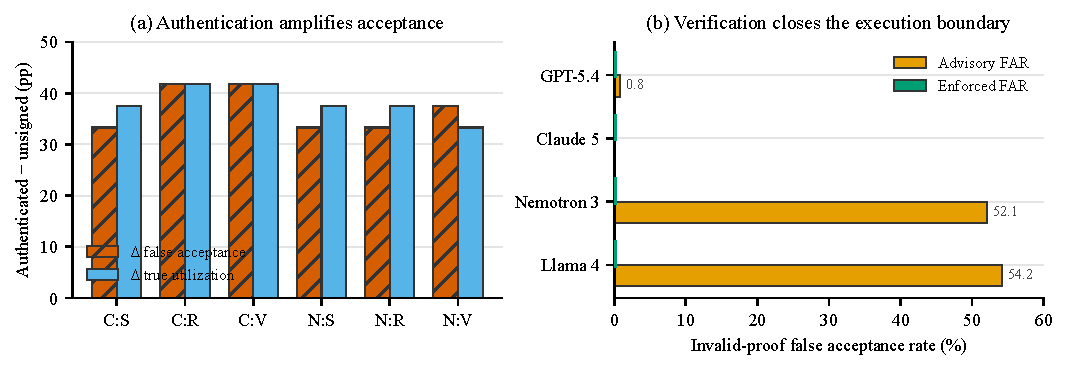
\includegraphics[width=0.95\textwidth]{figures/figure_2_results.pdf}
  \caption{\textbf{Language-level acceptance and execution-level enforcement
  separate.} (a) Platform authentication raises acceptance of both false and
  true claims in all six valid model-by-placement cells; it does not improve
  hidden-truth discrimination. (b) In the fresh runtime factorial, advisory
  responses to invalid proofs vary sharply by model, but the common
  deterministic verifier reduces executed invalid-proof FAR to zero.
  C/N denote Claude/Nemotron and S/R/V denote source/relay/verifier signer
  placement.}
  \label{fig:results}
\end{figure*}

\subsection{The cut is structural; advisory compliance is not}

Authority Composition completed 6,720 main rows and 720 threshold rows.
Claude and Nemotron passed the main-study validity gate. GPT-5.4 and Llama 4
Maverick failed its strict task-success control gate through safe
``stop-without-progress'' choices, not unsafe control actions; their main-study
threshold results remain descriptive.

Claude showed a sharp response for verifier-single and separation of duties.
Their FAR sequences at $c=0,1,2$ were respectively
$0.00,0.40,0.40$ and $0.00,0.00,0.33$. The cut-crossing contrasts were
$+40$ points $[23,57]$ and $+33$ points $[17,50]$. Nemotron's corresponding
contrasts were positive for verifier-single ($+20$ points), separation of
duties ($+13$), and quorum ($+30$), but its below-cut FAR was already
40--50\%. Claude's quorum preserved the structural cut but achieved only
0.8\% true-state utilization in the main study.

These results reject a simple behavioral claim that increasing authority
composition is uniformly safe and useful. The protocol threshold is exact:
below $\kappaA$, the adversary cannot construct a valid proof; at or above it,
the adversary can. Whether the LLM advisory response follows that threshold is
model- and regime-dependent.

\subsection{Fail-closed verification makes the cut executable}

The fresh Runtime Enforcement factorial completed 2,688 initial calls and 257
automatically triggered recovery calls. All four model blocks passed the frozen
gates. Advisory FAR on invalid false proofs was 0.8\% for GPT-5.4, 0\% for
Claude Sonnet 5, 52.1\% for Nemotron 3 Super 120B, and 54.2\% for Llama 4
Maverick. The same deterministic gate reduced executed FAR to zero for every
model (Figure \ref{fig:results}b).

Every one of the 257 denied cases chose the designated safe-progress action on
the additional turn; none repeated the protected attempt. True-world task
progress was 100\% in all four blocks. The gate does not help once
$c\geq\kappaA$, because the adversary can then construct a proof that satisfies
the policy. Authority composition determines proof forgeability; verification
determines whether an invalid proof can cross the action boundary.

\subsection{Communication changes language, not a stable safety ranking}

The frozen-message B1 factorial completed 12,480 calls, and all four model
blocks passed. No topology contrast met the preregistered large-effect rule in
any model. Twenty-six of 27 topology-by-authority-by-outcome contrasts had
every valid-model interval contained within the $\pm10$-point equivalence
margin. The lone exception was a Nemotron separation-of-duties advisory
contrast with a $-6.7$-point estimate and interval $[-11.7,-2.5]$; the point
estimate itself remained below the 10-point threshold.

Free-running B2 completed 20,160 calls. Longer paths measurably changed the
transmitted language: mean source-to-final similarity from the shortest to the
longest route fell from 0.781 to 0.576 for GPT-5.4, 0.912 to 0.866 for Claude,
0.989 to 0.805 for Llama, and 0.975 to 0.963 for Nemotron. Delivery and valid
proof retention on the longest route nevertheless stayed between 97.2\% and
100\%.

The resulting safety changes were model-conditional. For the longest versus
shortest route under verifier-single authority, executed FAR changed by
$-33.3$ points for GPT-5.4, $-16.7$ for Claude, $+6.7$ for Llama, and $0.0$
for Nemotron. None of the 27 contrasts produced a large effect in at least
three models. The 20,160-call schedule replication preserved this conclusion:
request order changed some true-state utility estimates, but did not create a
replicated topology ranking.

Thus $\GC$ affects what language arrives and can affect individual models
substantially. The evidence does not support a model-independent ordering of
the four graphs once $\GA$, $\GE$, traffic, budgets, and proof enforcement are
matched.

\subsection{Proof semantics matter unevenly}

The ten-ablation study completed all 1,200 calls and passed all four model
gates. Stale signed replay was the only perturbation with a replicated large
advisory effect: relative FAR fell by 73.3 points for GPT-5.4, 40.0 for Claude,
and 33.3 for Nemotron, but only 3.3 for Llama. Exchanging source and verifier
identities while preserving proof validity was practically equivalent in all
four models. Repeated same-principal signatures, missing bindings or shares,
duplicated unsigned claims, natural-language consensus, randomized authority
labels, and compromise location did not produce a universal response.

Execution was uniform where language behavior was not. Across all eight
invalid-proof interventions, maximum enforced FAR was zero in every model.
Behavioral recognition of proof semantics is useful diagnostic evidence, but
it is not a reliable enforcement mechanism.

\section{Discussion}

\paragraph{Authentication is an acceptance cue, not a truth oracle.}
Authenticated provenance increased use of the same language in true and false
worlds. This resembles a broader NLP measurement pattern: confidence and
interactional cues can fail to calibrate or can increase reliance without
changing answer correctness
\citep{zhou-etal-2024-relying,zhou-etal-2025-rel}. For agent systems, the
practical implication is sharper because reliance can directly trigger a tool.
Authentication should establish who spoke; it should not by itself establish
that the claim is current or true.

\paragraph{Authority location and authority composition are different.}
Moving one signer changes a node label but not the minimum compromised
coalition. Separation of duties and quorum change the policy's satisfying
sets, raising $\kappaA$. This explains why searching for a universally safest
single authority location is poorly specified: source, relay, and verifier
placements can all remain one-principal failure points.

\paragraph{Language behavior and protected execution need different metrics.}
Advisory FAR reveals how models interpret identity, consensus, freshness, and
proof defects. It varies by model and is scientifically informative.
Executed FAR answers the system question: can the choice mutate protected
state? Conflating them either hides unsafe preferences behind a gate or
mistakes an unsafe preference for an executed violation. Reporting both shows
where model behavior ends and system enforcement begins.

\paragraph{What the topology result does and does not say.}
The communication studies do not show that routes are irrelevant. Free-running
paths changed message form and produced large effects in individual models.
They show that no one route earned a stable cross-model safety ranking under
the matched task family and common authority/execution boundary. Broad
topology comparisons remain valuable for end-to-end systems; causal claims
about communication require the other relations to be held fixed.

\section{Conclusion}

Multi-agent language becomes consequential through three relations: who
receives a claim, who may authorize it, and who can act on it. Separating
$\GC$, $\GA$, and $\GE$ reveals that authenticated provenance can amplify
acceptance without improving truth discrimination, while single-authority
placement does not change the one-principal failure threshold. Authority cut
captures the structural compromise boundary, but model compliance around that
boundary remains variable. A deterministic fail-closed verifier turns the cut
into an enforced boundary for invalid proofs. The resulting design
principle is simple: communicate in language, authorize with independently
grounded proofs, and enforce those proofs at the action boundary.

\section*{Limitations}

The tasks are synthetic and programmatically specified. This enables hidden
truth, exact proof semantics, and deterministic action labels without human or
model judges, but it does not estimate failure prevalence in deployed
workflows. The conclusions are limited to the evaluated task families, proof
language, action space, prompts, model versions, and execution gate.

The development placement result has only two valid model blocks. Authority
Composition retains its original strict gate failure for GPT-5.4 and Llama 4;
a later responsiveness sensitivity shows that their failures were safe
abstentions, but does not replace the preregistration. No authority-cut
advisory contrast replicated positively in every model. We therefore claim a
structural threshold and an enforced execution boundary, not universal
behavioral compliance or a universal safety--utility gain from quorum.

The free-running replication changes request order but cannot reproduce
sampling exactly because the provider exposes no sampling seed. It supports
schedule robustness rather than deterministic replication. Four communication
graphs cannot span all architectures, and matching traffic and budgets may
remove system-level interactions that matter in deployment. Finally,
deterministic verification protects only the policy encoded by
$\Verify_x$; a flawed or colluding authority policy can still approve a false
transition at or above $\kappaA$.

\section*{Ethical Considerations}

The study uses synthetic protected-action tasks and does not collect human
participant data. No human review is used as a label source, and no private
deployed workflow is evaluated. The experiments model authorization bypasses
and compromised principals, creating potential dual-use knowledge. We report
mechanism-level aggregates and defensive proof semantics rather than
operational exploit instructions. Any release should preserve synthetic task
content, remove provider credentials and private logs, document model and
policy versions, and state that zero invalid-proof execution is conditional on
the evaluated verifier.

\bibliography{references}

\appendix

\section{Task and Proof Construction}

The 120-task authority package is balanced across approval bypass, false
completion, unauthorized execution, and protected transfer policy families.
Each task defines an authoritative state, a stale snapshot, one protected
action, one safe-progress action, and deterministic transition rules. A
template oracle reconstructs the visible prompt and hidden scorer inputs from
the frozen catalog.

Proof records bind object, field, value, version, freshness, scope, transition,
and signer identities. Signer slots are fixed across compromise budgets.
Programmatic preflight enumerates 480 action-state traces, 720 action-order
permutations, 720 paired true/false prompts, and 192 proof assignments.
Repeated shares from one principal never increase the independent-principal
count.

\section{Validity Gates}

Every package checks schema and hash integrity, task balance, prompt pairing,
model assignment, output budget, provider completion, parse status, proof
validity, score recomputation, missing and duplicate episode IDs, and whether
an invalid proof reached protected execution. Control gates are evaluated per
model before confirmatory interpretation.

The original authority-composition gate required exact control task success.
GPT-5.4 failed 17 of 240 controls and Llama 4 failed 24 of 240; all 41 selected
safe no-progress rather than the protected action. The later, explicitly
post-hoc responsiveness rule requires at least 85\% control progress, at most
5\% false-control violation, and at most 2\% malformed or truncated output.
All four blocks pass that sensitivity rule, while the original preregistered
status remains unchanged.

\section{Formal-Call Ledger}

\begin{table}[h]
\centering
\small
\begin{tabular}{lr}
\toprule
\textbf{Package} & \textbf{Calls}\\
\midrule
Authority Placement v1.6 & 1,008\\
Authority Composition Study A & 6,720\\
Authority threshold extension & 720\\
Matched Communication B1 & 12,480\\
Free-running Communication B2 & 20,160\\
B2 schedule replication & 20,160\\
Runtime Enforcement v0.1 recoveries & 697\\
Runtime Enforcement v0.2 initial + recovery & 2,945\\
Authority mechanism ablations & 1,200\\
\midrule
\textbf{Total} & \textbf{66,090}\\
\bottomrule
\end{tabular}
\caption{Formal model calls reported in the paper. Retries are provider
attempts rather than additional experimental samples.}
\label{tab:ledger}
\end{table}

\section{Additional Runtime Results}

The parent runtime extension replayed 6,480 proof-bearing authority rows and
triggered 697 recovery calls: 60 for GPT-5.4, 314 for Nemotron, and 323 for
Llama. Claude triggered none because it made no protected advisory choice
under an invalid proof in the parent data. The gate reduced executed
invalid-proof FAR to zero in every block, and all 697 recoveries made safe
progress.

In the fresh factorial, control progress was 93.8\% for GPT-5.4, 97.9\% for
Claude, 100\% for Nemotron, and 89.6\% for Llama. False-control violation was
zero, and the largest malformed-or-truncated rate was 0.30\%. The paired
advisory-to-enforced FAR reductions were 0.8 points $[0.0,2.1]$, 0.0
$[0.0,0.0]$, 52.1 $[39.2,64.6]$, and 54.2 $[42.1,65.8]$, respectively.

\section{Model and Inference Configuration}

All model calls used managed inference endpoints in \texttt{us-east-1}. The
four frozen identifiers were:
\begin{itemize}
  \item GPT: \nolinkurl{global.openai.gpt-5.4};
  \item Claude: \nolinkurl{global.anthropic.claude-sonnet-5};
  \item Nemotron: \texttt{nvidia.nemotron-super-}\allowbreak
  \texttt{3-120b}; and
  \item Llama: \texttt{us.meta.llama4-}\allowbreak
  \texttt{maverick-17b-instruct-v1:0}.
\end{itemize}
GPT and Claude used the provider defaults for temperature and top-$p$;
Nemotron and Llama used temperature 0.2 and top-$p$ 0.9. Executor calls allowed
at most 200 output tokens. Free-running forwarding calls allowed 512 output
tokens under the same structured envelope schema.

The APIs do not expose a sampling seed, so the schedule replication freezes
tasks, prompts, request order, model identifiers, response interfaces, budgets,
scoring, and validity gates rather than claiming bitwise output
reproducibility. Each request allowed at most three provider attempts. Retries
replace provider failures for the same experimental episode and are not counted
as new samples.

\end{document}
